\documentclass{ijclclp}
\usepackage{hyperref}
\usepackage{xcolor}
\usepackage{caption}
\usepackage{subcaption}
\usepackage{enumitem}

\title{The Coin Flip Judge: Quantifying Inconsistency and Position Bias in LLM-as-a-Judge Evaluation}
\author{Abel Yagubyan\textsuperscript{1}}
\affiliation{Independent Researcher}
\email{\texttt{abel.yagubyan@gmail.com}}

\begin{document}
\maketitle
\thispagestyle{firstpage}

\begin{abstract}
LLM-as-a-Judge has become the dominant paradigm for evaluating language model outputs, yet its reliability under repeated trials remains insufficiently characterized. We present a reproducibility study examining the internal consistency of two OpenAI judge models---GPT-4o-mini and GPT-4.1-mini---across 29 diverse evaluation tasks spanning 10 categories. Each task is judged 50 times in both pairwise comparison and pointwise scoring modes, yielding 8,700 total judgments, supplemented by temperature and prompt sensitivity ablations totaling over 10,000 evaluations. We find that (1) pairwise preferences flip 14\% of the time on average when response order is randomized, with some questions reaching 56\% flip rates---worse than a coin flip; (2) strong position bias exists, with first-position (A) responses winning majority preference in 72\% of questions for GPT-4o-mini ($p = 0.024$, sign test); (3) pointwise scores are nearly identical between responses (mean gap $= 0.19$--$0.36$ points on a 10-point scale), yet judges still confidently declare ``winners'' in pairwise mode; and (4) cross-judge agreement reaches only 76\% (Cohen's $\kappa = 0.51$), with disagreements concentrated in subjective and coding tasks. A temperature ablation study shows that setting $t=0$ reduces but does not eliminate inconsistency, with GPT-4.1-mini still exhibiting 7.9\% mean flip rates under deterministic decoding. A prompt sensitivity analysis further reveals that semantically equivalent but differently worded prompts change the majority outcome in 25\% of cases. These findings suggest that LLM judges may be less stable than commonly assumed, with implications for leaderboard rankings, RLHF reward modeling, and benchmark design.

\\
\\
\textbf{Keywords:} LLM evaluation, LLM-as-a-Judge, position bias, evaluation reliability, pairwise comparison, benchmark design
\end{abstract}

\section{Introduction}

The rapid proliferation of large language models (LLMs) has created an acute need for scalable evaluation methods. Human evaluation, while considered the gold standard, is expensive, slow, and itself subject to well-documented biases \citep{clark2021all}. This has driven widespread adoption of LLM-as-a-Judge frameworks, where a capable language model evaluates the outputs of other models \citep{zheng2023judging}.

Major evaluation platforms including Chatbot Arena \citep{chiang2024chatbot}, AlpacaEval \citep{dubois2024alpacafarm}, and MT-Bench \citep{zheng2023judging} now rely on LLM judges as primary or supplementary evaluators. RLHF pipelines use LLM judges as reward model proxies \citep{ouyang2022training, bai2022constitutional}. Yet a fundamental question remains underexplored: \textit{how consistent are these judges with themselves?}

Prior work has identified position bias \citep{wang2023large, zheng2023judging}, verbosity bias \citep{zheng2023judging}, and self-enhancement bias \citep{zheng2023judging} in LLM judges. However, these studies primarily examine biases through single-trial or small-sample experiments, and focus on \textit{inter-rater} or \textit{inter-model} agreement rather than the \textit{intra-rater} consistency of a single judge across repeated identical evaluations. The stochastic nature of LLM generation---even at low temperatures---means that repeated evaluations of identical inputs may yield different outcomes, yet this source of variance has received limited systematic attention.

We build on this prior work by providing a focused, large-scale study of intra-judge consistency. While \citet{stureborg2024large} characterize bias across a broad range of conditions, our study is distinguished by its combination of 50-trial pairwise flip rates, the pairwise-pointwise paradox analysis, controlled temperature ablation, and prompt sensitivity experiments on a single cohesive dataset. Specifically, we measure:

\begin{itemize}[nosep]
    \item \textbf{Flip rate}: How often does a judge change its pairwise preference when re-evaluated?
    \item \textbf{Position bias}: Does presentation order systematically influence preferences?
    \item \textbf{Pairwise-pointwise disconnect}: Do judges that give identical scores still declare winners?
    \item \textbf{Cross-judge agreement}: Do different judge models agree on the same evaluations?
    \item \textbf{Temperature sensitivity}: Does deterministic decoding ($t=0$) eliminate inconsistency?
    \item \textbf{Prompt sensitivity}: Does the wording of the evaluation prompt affect outcomes?
\end{itemize}

Our results reveal notable levels of inconsistency that warrant caution when interpreting single-trial LLM judge evaluations.

\section{Related Work}

\subsection{LLM-as-a-Judge}

\citet{zheng2023judging} introduced MT-Bench and demonstrated that GPT-4 judgments correlate well with human preferences in aggregate, while identifying position and verbosity biases. \citet{dubois2024alpacafarm} proposed AlpacaFarm for instruction-following evaluation, showing that LLM judges can approximate human annotators at lower cost.

\subsection{Bias in LLM Evaluation}

\citet{wang2023large} conducted a systematic study of LLM judge biases, finding significant position bias and self-enhancement tendencies across multiple models. \citet{stureborg2024large} found that LLM judges are influenced by superficial features like response length and formatting. \citet{liu2023geval} proposed G-Eval, showing that chain-of-thought prompting improves judge calibration but does not resolve stochastic variance between runs.

\subsection{Evaluation Reliability and Human Baselines}

\citet{zhu2023judgelm} proposed JudgeLM for training dedicated judge models. \citet{shankar2024validates} questioned who validates the validators, highlighting the circularity of using LLMs to evaluate LLMs.

For context, human inter-annotator agreement on subjective NLG evaluation tasks typically ranges from $\kappa = 0.3$--$0.6$ \citep{amidei2019agreement}, with pairwise preference tasks achieving $\kappa = 0.4$--$0.7$ depending on task subjectivity \citep{clark2021all}. \citet{zheng2023judging} reported that MT-Bench human agreement on pairwise preferences was approximately 81\%, and Chatbot Arena crowdworker agreement was around 66\% \citep{chiang2024chatbot}. Our work complements these studies by focusing specifically on \textit{intra-judge consistency}---the reliability of a single judge across repeated evaluations of identical inputs---and providing direct comparisons to these human baselines.

\section{Methodology}

\subsection{Evaluation Dataset}

We construct a diverse evaluation set of 29 question-response pairs spanning 10 categories: writing (3), reasoning (3), coding (3), knowledge (3), math (3), roleplay (2), extraction (3), ethics (2), instruction-following (3), and hard/ambiguous tasks (4). For each question, we use two high-quality responses from different model tiers (GPT-4o-mini and GPT-4o) to ensure meaningful comparison targets.

Response pairs are deliberately chosen to be competitive---both responses are high-quality but differ in style, structure, or approach. Pointwise evaluation confirms this: across both judges, Response A averages $9.3/10$ ($\sigma = 0.9$) and Response B averages $9.4/10$ ($\sigma = 0.6$), indicating that both responses are consistently rated as high-quality. This design maximizes the sensitivity of our consistency measurements; trivially different responses would yield artificially high consistency. We note that this represents a stress test: real-world evaluation often involves more diverse quality levels, and consistency may be higher for response pairs with obvious quality differences.

\subsection{Judge Models}

We evaluate two judge models from the GPT-4 family:
\begin{itemize}[nosep]
    \item \textbf{GPT-4o-mini}: A cost-efficient model commonly used for large-scale evaluation
    \item \textbf{GPT-4.1-mini}: A newer variant from the GPT-4.1 family
\end{itemize}

Both models are accessed through the OpenAI API. The main experiment uses the default temperature ($t=1.0$) to reflect real-world usage; a supplementary ablation study evaluates $t=0$ (deterministic decoding).

\subsection{Evaluation Protocol}

\textbf{Experiment 1 (Main).} For each (judge, question) pair, we conduct:

\begin{enumerate}[nosep]
    \item \textbf{Pairwise comparison} ($\times 50$): The judge is asked ``Which response is better?'' with randomized A/B presentation order across trials.
    \item \textbf{Pointwise scoring} ($\times 50$ per response): Each response is independently scored on a 1--10 scale.
\end{enumerate}

This yields $29 \times 2 \times (50 + 50 + 50) = 8{,}700$ total API calls. The 50-trial design provides sufficient statistical power to distinguish genuine preferences from noise (binomial test $p < 0.05$ requires $\geq 33/50$ for significance).

\textbf{Experiment 2 (Temperature Ablation).} We repeat the pairwise comparison with $t=0$ for 10 trials per (judge, question) pair, yielding an additional $29 \times 2 \times 10 = 580$ API calls. While $t=0$ should theoretically produce deterministic outputs, API-level factors (batching, quantization, floating-point nondeterminism) may introduce variation.

\textbf{Experiment 3 (Prompt Sensitivity).} We design a second, semantically equivalent prompt template with different framing and structure, and evaluate 10 diverse questions (one per category) with 20 trials per (judge, prompt, question) combination, yielding $10 \times 2 \times 2 \times 20 = 800$ additional API calls.

\subsection{Metrics}

\textbf{Flip Rate.} For each question, we define the flip rate as:
\begin{equation}
    \text{FR} = 1 - \frac{\max(n_A, n_B, n_{\text{tie}})}{N}
\end{equation}
where $n_A$, $n_B$, $n_{\text{tie}}$ are the counts of each outcome across $N$ trials. A flip rate of 0\% indicates perfect consistency; 50\% indicates random behavior.

\textbf{Position Bias Index.} We measure the fraction of questions where response A (presented first) wins the majority vote:
\begin{equation}
    \text{PBI} = \frac{|\{q : \text{majority}(q) = A\}|}{|\mathcal{Q}|}
\end{equation}
An unbiased judge would yield PBI $\approx 0.5$. We test significance using a sign test.

\textbf{Pairwise-Pointwise Gap.} For each question, we compute:
\begin{equation}
    \text{PPG} = |\bar{s}_A - \bar{s}_B|
\end{equation}
where $\bar{s}_A$ and $\bar{s}_B$ are mean pointwise scores across 50 trials. We test whether aggregate pointwise scores differ using the Wilcoxon signed-rank test.

\textbf{Cross-Judge Agreement.} We report both raw agreement percentage and Cohen's $\kappa$ to account for chance agreement.

All confidence intervals are computed via bootstrap resampling (10,000 iterations).

\section{Results}

\subsection{Intra-Judge Consistency}

\begin{table}[h]
\centering
\caption{Summary of judge consistency metrics across 29 evaluation tasks ($t=1.0$). FR = Flip Rate, PBI = Position Bias Index. 95\% CIs computed via bootstrap.}
\label{tab:summary}
\begin{tabular}{lcc}
\toprule
\textbf{Metric} & \textbf{GPT-4o-mini} & \textbf{GPT-4.1-mini} \\
\midrule
Mean FR (\%) & 13.3 [7.7, 19.4] & 13.9 [7.7, 20.3] \\
Median FR (\%) & 4.0 & 6.0 \\
Max FR (\%) & 46.0 & 56.0 \\
FR $>$ 20\% & 8/29 (28\%) & 8/29 (28\%) \\
FR $=$ 0\% & 8/29 (28\%) & 10/29 (34\%) \\
PBI (A majority) & 72\% ($p=0.024$) & 59\% ($p=0.458$) \\
Mean PPG & 0.19 & 0.36 \\
\bottomrule
\end{tabular}
\end{table}

Table~\ref{tab:summary} presents aggregate consistency statistics. Both judges exhibit mean flip rates of approximately 14\%, indicating that roughly one in seven evaluations would change if re-run. However, the distribution is highly bimodal (Figure~\ref{fig:flip_rates}): many questions show near-perfect consistency (FR $= 0$\%), while others approach coin-flip territory. The two judges do not differ significantly in overall flip rate (Mann-Whitney $U = 438$, $p = 0.783$).

\begin{figure}[h]
    \centering
    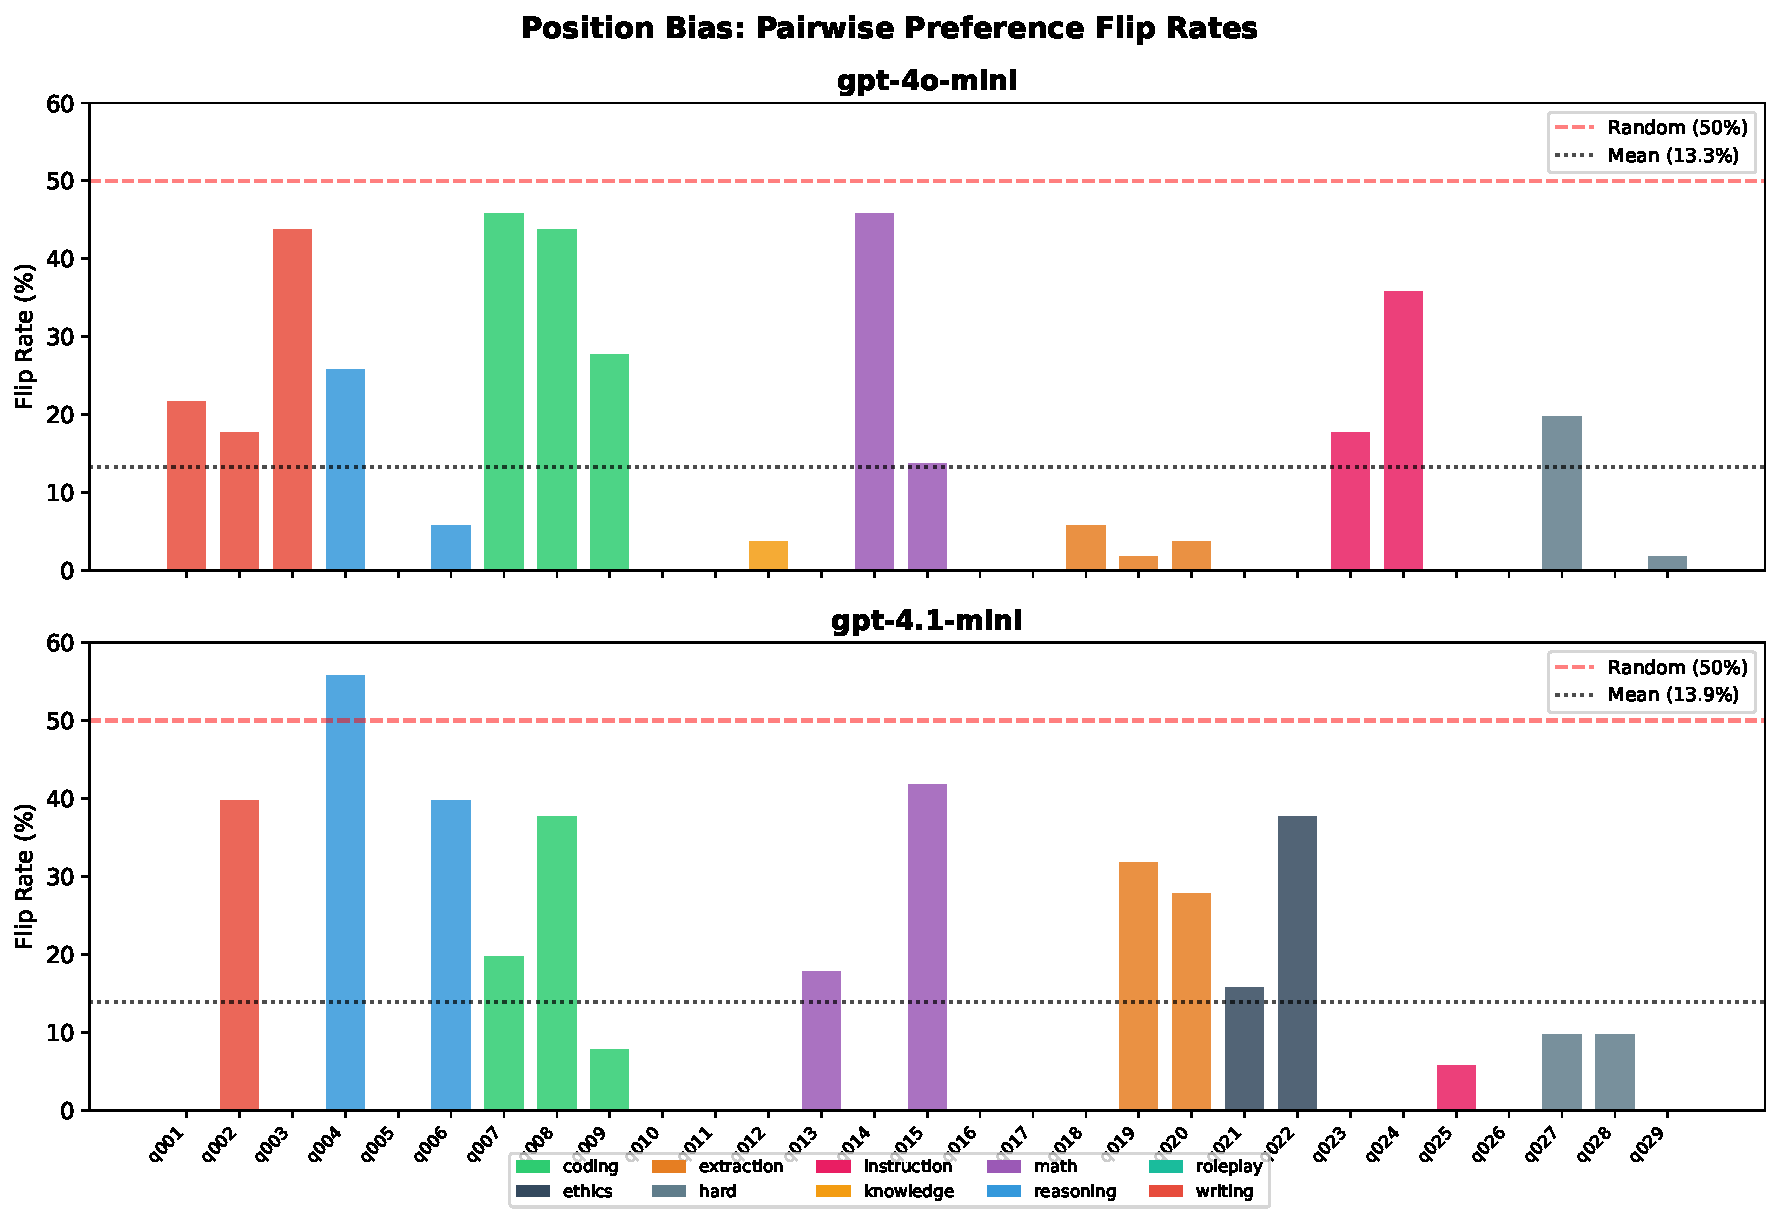
\includegraphics[width=\linewidth]{figures/fig1_flip_rates.pdf}
    \caption{Pairwise preference flip rates across 29 questions for each judge model. Dashed red line indicates random baseline (50\%). Color indicates task category.}
    \label{fig:flip_rates}
\end{figure}

The most notable finding is the existence of extreme inconsistency: GPT-4.1-mini achieves a 56\% flip rate on q004 (a reasoning task), meaning its preferences are \textit{less consistent than random coin flips}. Eight questions per judge exceed 20\% flip rates, concentrated in coding (39\% mean for GPT-4o-mini), writing, and reasoning categories.

\subsection{Position Bias}

\begin{figure}[h]
    \centering
    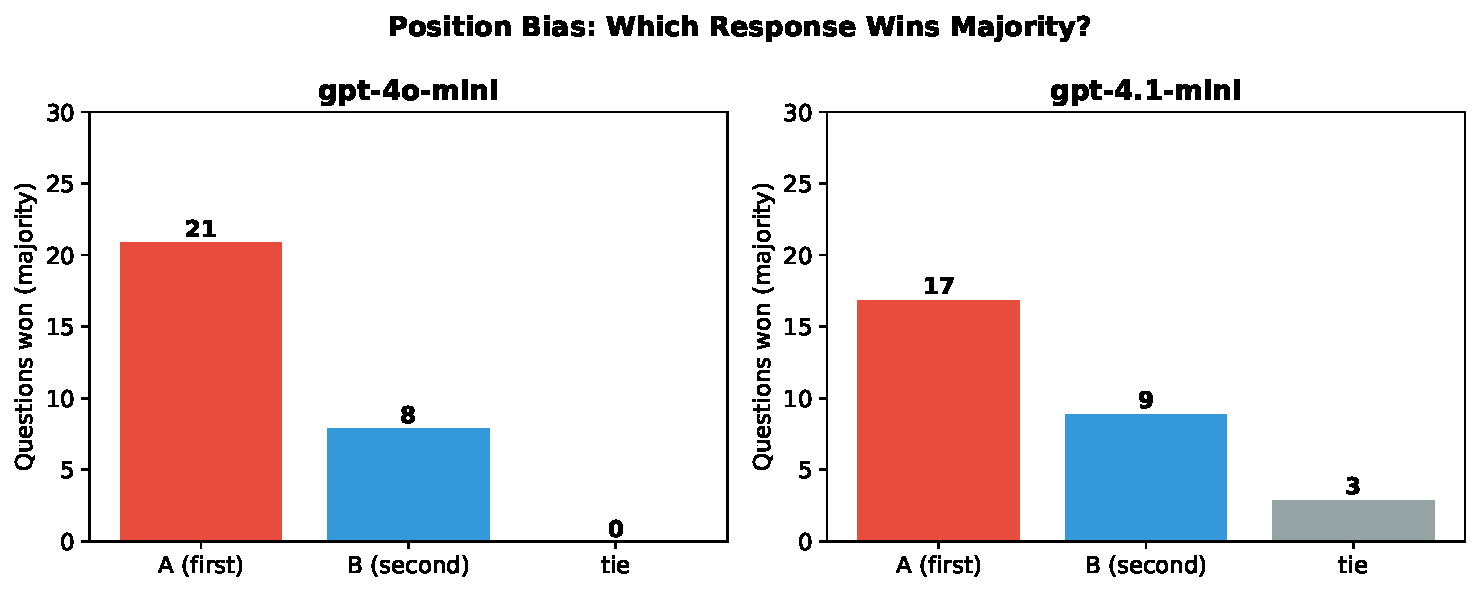
\includegraphics[width=0.85\linewidth]{figures/fig2_position_bias.pdf}
    \caption{Distribution of majority preference by position. An unbiased judge would show roughly equal A and B wins.}
    \label{fig:position_bias}
\end{figure}

Figure~\ref{fig:position_bias} reveals substantial position bias. GPT-4o-mini shows a strong primacy effect, with the first-presented response (A) winning majority preference in 21 of 29 questions (72\%, sign test $p = 0.024$). GPT-4.1-mini is more balanced at 59\% ($p = 0.458$, not significant). At the individual question level, 24 of 29 questions show significant position bias ($p < 0.05$, binomial test) for \textit{both} judges, indicating that position effects are pervasive even when aggregate bias appears moderate.

This position bias has direct implications for evaluation fairness: a model whose response happens to appear first will systematically receive more favorable evaluations.

\subsection{The Pairwise-Pointwise Paradox}

\begin{figure}[h]
    \centering
    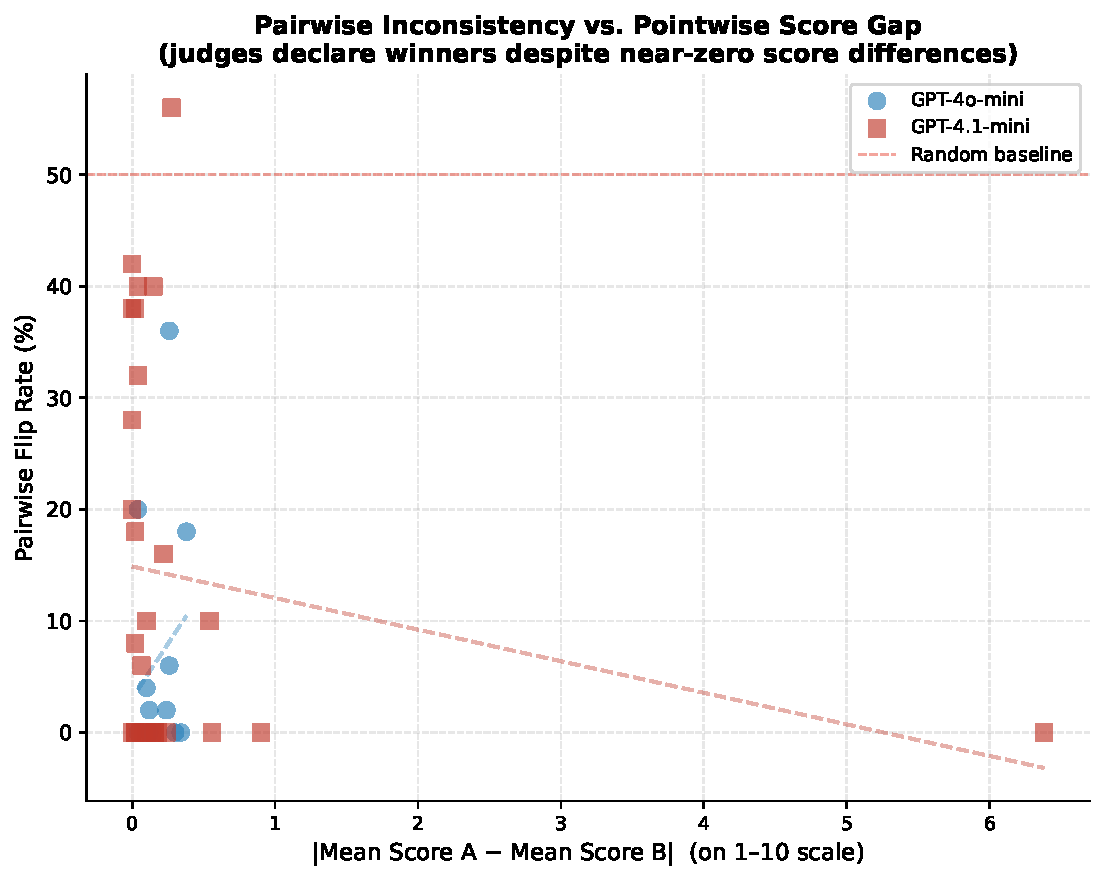
\includegraphics[width=0.85\linewidth]{figures/fig4_score_vs_flip.pdf}
    \caption{Relationship between pointwise score gap and pairwise flip rate. Many high-flip-rate questions have near-zero score differences.}
    \label{fig:paradox}
\end{figure}

Perhaps the most notable finding is the disconnect between pairwise preferences and pointwise scores. The mean pointwise score gap is only 0.19 points for GPT-4o-mini and 0.36 for GPT-4.1-mini on a 10-point scale. Crucially, aggregate pointwise scores do \textit{not} significantly differ between responses A and B for either judge (Wilcoxon signed-rank: GPT-4o-mini $W=42$, $p=0.827$; GPT-4.1-mini $W=96.5$, $p=0.126$). Yet in pairwise mode, the same judges confidently pick ``winners.''

Figure~\ref{fig:paradox} illustrates this paradox. Questions with near-zero score differences often exhibit high flip rates, suggesting the judge is essentially guessing when forced to choose between equally-rated responses. This finding challenges the common practice of interpreting pairwise preferences as indicating meaningful quality differences.

\subsection{Category Analysis}

\begin{figure}[h]
    \centering
    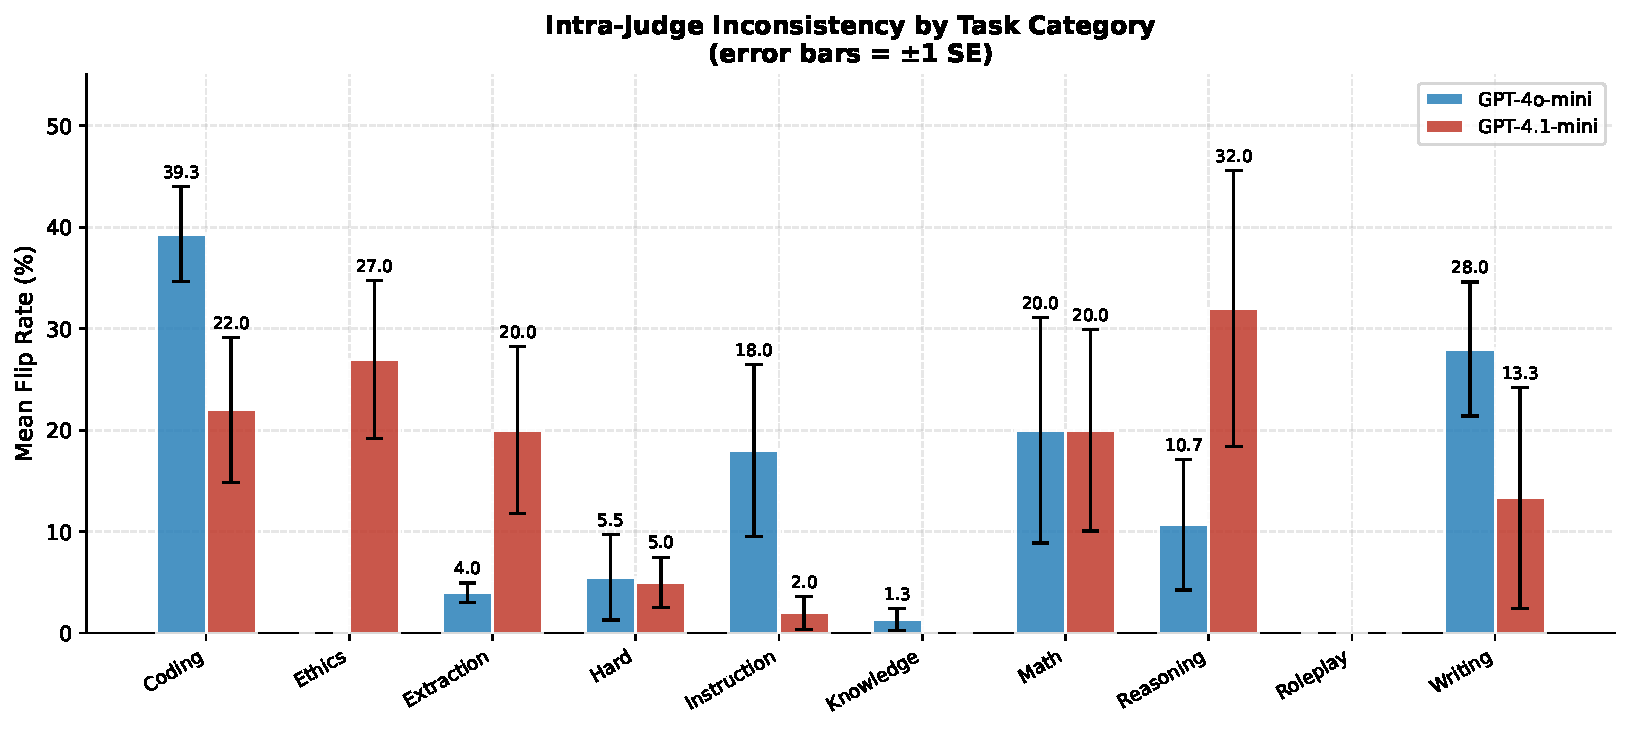
\includegraphics[width=\linewidth]{figures/fig3_category_flips.pdf}
    \caption{Mean flip rate by task category for each judge. Categories with subjective evaluation criteria show higher inconsistency.}
    \label{fig:categories}
\end{figure}

Figure~\ref{fig:categories} shows flip rates broken down by task category. While there is a trend toward higher inconsistency in subjective categories (coding, writing, reasoning) compared to factual ones (knowledge, roleplay), the differences do not reach statistical significance (Kruskal-Wallis: GPT-4o-mini $H=15.8$, $p=0.071$; GPT-4.1-mini $H=11.4$, $p=0.252$), likely due to the small number of questions per category.

The pattern differs substantially between judges:

\begin{itemize}[nosep]
    \item \textbf{Coding}: High inconsistency for GPT-4o-mini (39\%) but moderate for GPT-4.1-mini (22\%)
    \item \textbf{Reasoning}: Moderate for GPT-4o-mini (11\%) but high for GPT-4.1-mini (32\%)
    \item \textbf{Knowledge/Roleplay}: Consistently low flip rates ($<$5\%) for both judges
    \item \textbf{Ethics}: Stable for GPT-4o-mini (0\%) but variable for GPT-4.1-mini (27\%)
\end{itemize}

This category-dependent inconsistency suggests that judge reliability varies substantially by task type, and that the \textit{pattern} of unreliability differs across judges---a finding relevant for evaluation pipelines that use a single judge.

\subsection{Difficulty-Stratified Analysis}

To assess whether inconsistency is primarily driven by ambiguous questions, we stratify questions by difficulty, defined as the mean flip rate across both judges. Questions with mean FR $< 10\%$ are classified as ``easy'' (clear winner), while those with FR $\geq 10\%$ are ``hard'' (ambiguous).

\begin{table}[h]
\centering
\caption{Flip rates stratified by question difficulty. Easy questions show near-deterministic behavior; hard questions exhibit substantial instability.}
\label{tab:difficulty}
\begin{tabular}{lccc}
\toprule
\textbf{Stratum} & \textbf{N} & \textbf{Mean FR} & \textbf{Categories} \\
\midrule
Easy (FR $<$ 10\%) & 14 & 2.9\% & knowledge, roleplay, extraction \\
Hard (FR $\geq$ 10\%) & 15 & 23.6\% & coding, writing, reasoning \\
\bottomrule
\end{tabular}
\end{table}

Table~\ref{tab:difficulty} reveals a strongly bimodal distribution: nearly half of questions (14/29) are judged with high consistency (mean FR = 2.9\%), while the remaining 15 questions exhibit substantial instability (mean FR = 23.6\%). Easy questions cluster in factual and well-defined categories (knowledge, roleplay, extraction), while hard questions concentrate in subjective or open-ended categories (coding, writing, reasoning). This suggests that LLM judge inconsistency is not uniformly distributed but rather concentrated in task types where evaluation criteria are inherently more subjective---a pattern also observed in human annotation studies \citep{amidei2019agreement}.

\subsection{Cross-Judge Agreement}

\begin{figure}[h]
    \centering
    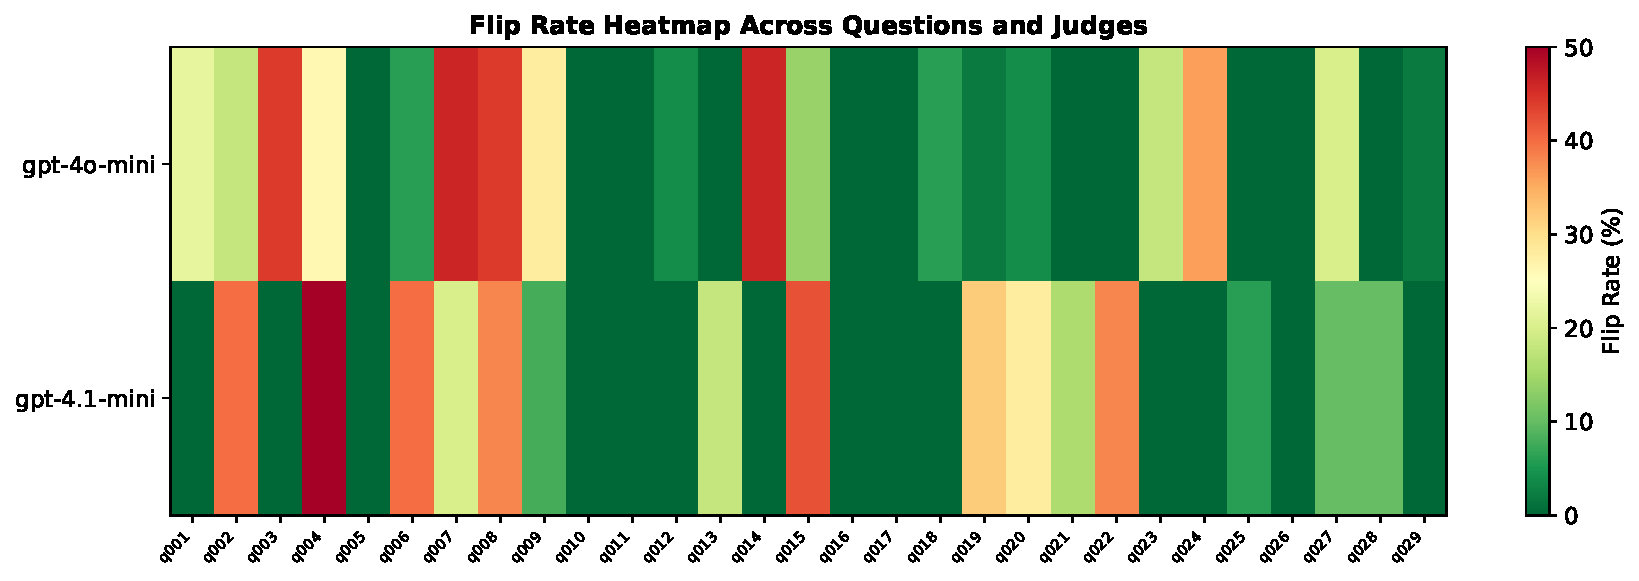
\includegraphics[width=\linewidth]{figures/fig5_heatmap.pdf}
    \caption{Flip rate heatmap across all questions and judges. Darker colors indicate higher inconsistency.}
    \label{fig:heatmap}
\end{figure}

The two judges agree on the majority-preferred response for only 22 of 29 questions (76\%), yielding Cohen's $\kappa = 0.51$ (moderate agreement). Disagreements are concentrated in writing (q002, q003), coding (q007, q008, q009), and hard tasks (q028). In three cases, GPT-4.1-mini declares a tie while GPT-4o-mini picks a winner, suggesting different decision thresholds.

For context, this $\kappa = 0.51$ is comparable to the lower end of human inter-annotator agreement on subjective NLG tasks ($\kappa = 0.3$--$0.6$; \citealt{amidei2019agreement}) and notably below the 81\% agreement reported for MT-Bench human evaluators \citep{zheng2023judging}. The 76\% inter-judge agreement rate means that approximately one in four evaluation outcomes depends on which judge model is selected.

\subsection{Temperature Ablation}

\begin{figure}[h]
    \centering
    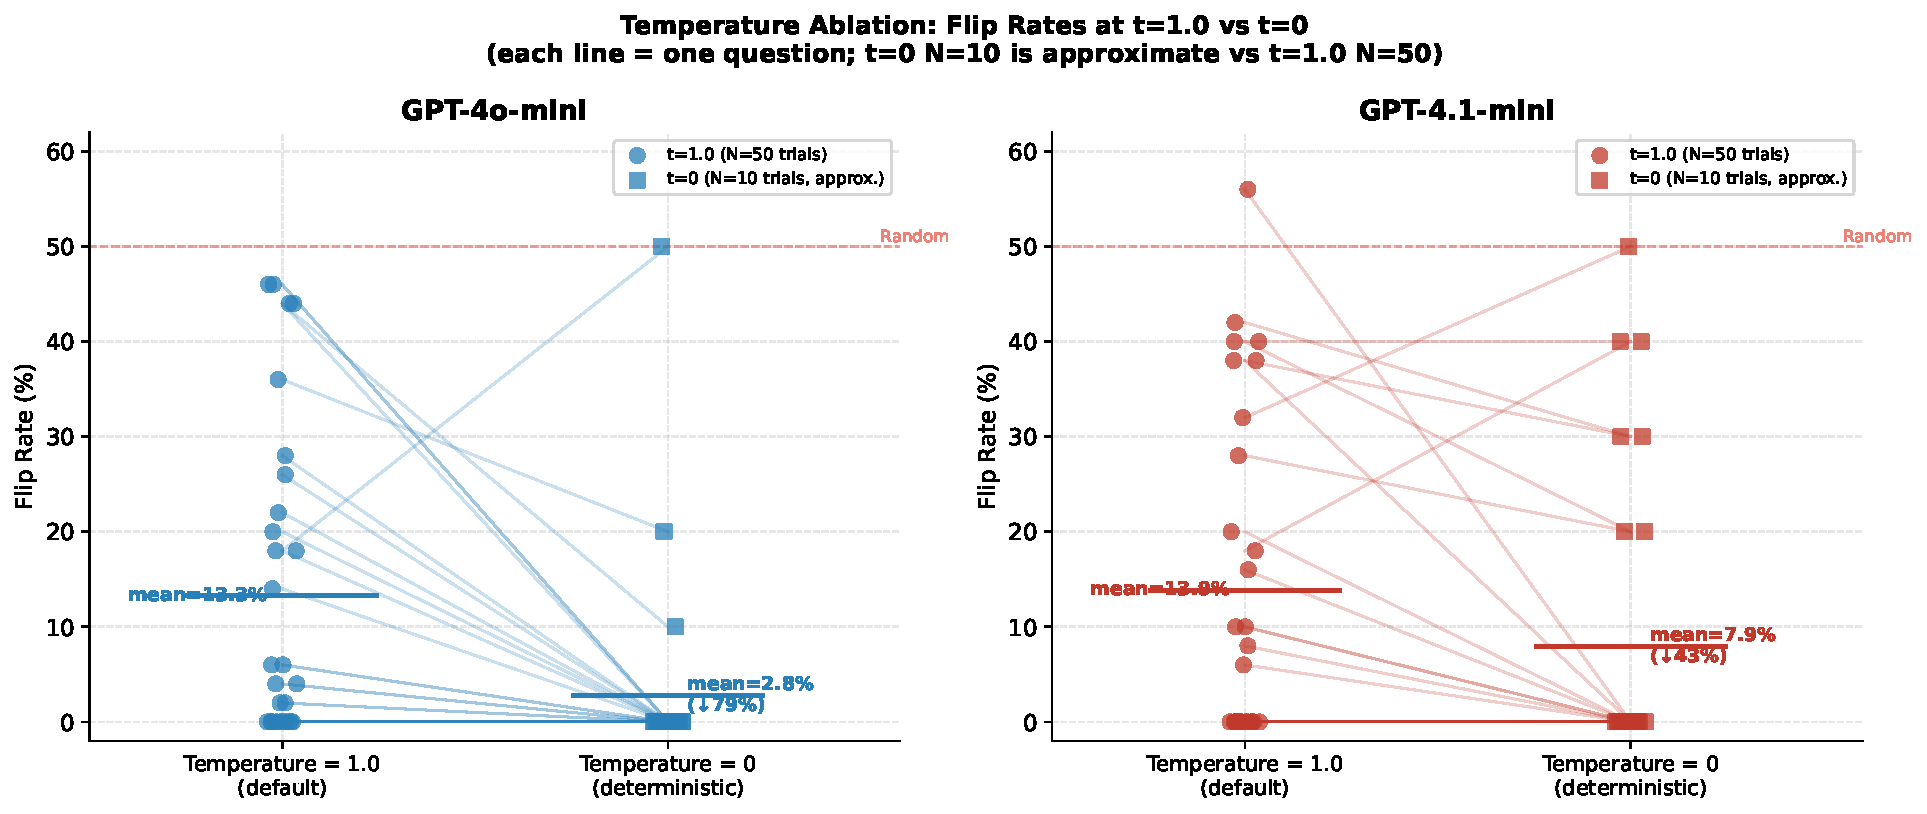
\includegraphics[width=\linewidth]{figures/fig6_temp_ablation.pdf}
    \caption{Flip rate comparison between $t=1.0$ (50 trials) and $t=0$ (10 trials). Deterministic decoding substantially reduces but does not eliminate inconsistency.}
    \label{fig:temp}
\end{figure}

\begin{table}[h]
\centering
\caption{Temperature ablation results. Flip rates at $t=0$ vs $t=1.0$.}
\label{tab:temp}
\begin{tabular}{lccc}
\toprule
\textbf{Judge} & \textbf{FR ($t=1.0$)} & \textbf{FR ($t=0$)} & \textbf{Reduction} \\
\midrule
GPT-4o-mini & 13.3\% & 2.8\% & 79\% \\
GPT-4.1-mini & 13.9\% & 7.9\% & 43\% \\
\bottomrule
\end{tabular}
\end{table}

Figure~\ref{fig:temp} and Table~\ref{tab:temp} present the temperature ablation results. Setting $t=0$ substantially reduces flip rates for GPT-4o-mini (79\% reduction, from 13.3\% to 2.8\%) but is less effective for GPT-4.1-mini (43\% reduction, to 7.9\%). Even at $t=0$, GPT-4.1-mini exhibits non-zero flip rates on 7 of 29 questions, with one reaching 50\%.

This residual inconsistency at $t=0$ likely reflects API-level nondeterminism (floating-point variations, batch processing effects) rather than intentional sampling. It demonstrates that \textbf{deterministic decoding is necessary but not sufficient} for consistent evaluation, and that additional strategies (multi-trial voting, multi-judge panels) remain important even when temperature is controlled.

\subsection{Prompt Template Sensitivity}

\begin{figure}[h]
    \centering
    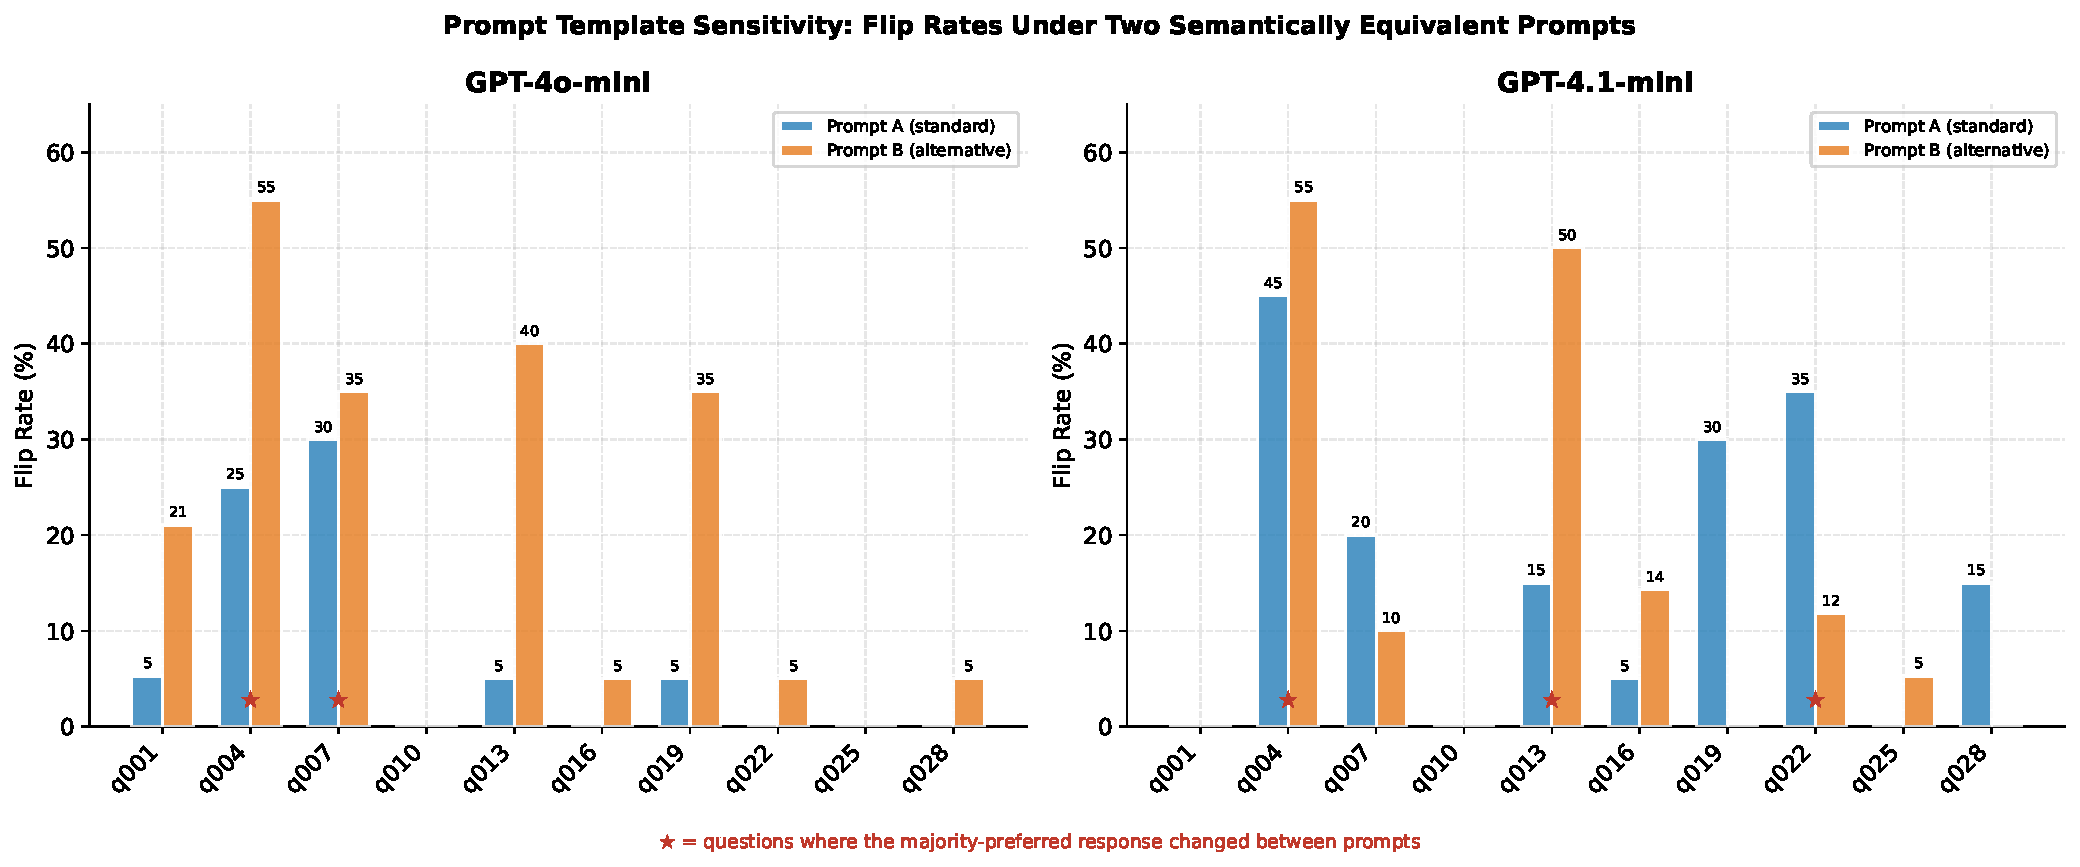
\includegraphics[width=\linewidth]{figures/fig7_prompt_sensitivity.pdf}
    \caption{Flip rates under two different prompt templates (20 trials each) on a 10-question subset. Prompt wording affects both consistency and majority preference.}
    \label{fig:prompt}
\end{figure}

To assess sensitivity to prompt wording, we designed two semantically equivalent but stylistically different evaluation prompts and tested them on a 10-question subset (20 trials each, both judges). Prompt A uses our standard format (``You are an impartial judge...''), while Prompt B uses an alternative framing (``Please act as a fair and unbiased evaluator...'' with step-by-step instructions).

\begin{table}[h]
\centering
\caption{Prompt template sensitivity on a 10-question subset. Cross-prompt agreement measures whether the majority-preferred response is the same under both prompts.}
\label{tab:prompt}
\begin{tabular}{lccc}
\toprule
\textbf{Judge} & \textbf{Cross-prompt} & \textbf{Mean $\Delta$FR} \\
 & \textbf{agreement} & \\
\midrule
GPT-4o-mini & 8/10 (80\%) & 11.6\% \\
GPT-4.1-mini & 7/10 (70\%) & 15.2\% \\
Combined & 15/20 (75\%) & 13.4\% \\
\bottomrule
\end{tabular}
\end{table}

As shown in Figure~\ref{fig:prompt} and Table~\ref{tab:prompt}, changing the prompt template flips the majority-preferred response in 25\% of cases (5/20), with an average absolute change in flip rate of 13.4 percentage points. Prompt B generally induces higher inconsistency, particularly for questions that were already borderline under Prompt A. This finding demonstrates that evaluation outcomes are sensitive not only to temperature and judge model, but also to the specific wording of the evaluation prompt---an often-overlooked source of variance.

\section{Discussion}

\subsection{Comparison to Human Annotators}

A natural question is whether LLM judges are more or less consistent than human evaluators. Table~\ref{tab:human} contextualizes our findings against reported human baselines.

\begin{table}[h]
\centering
\caption{LLM judge consistency vs.\ reported human baselines.}
\label{tab:human}
\begin{tabular}{lcc}
\toprule
\textbf{Evaluator} & \textbf{Agreement} & \textbf{Source} \\
\midrule
Human (MT-Bench pairwise) & 81\% & \citet{zheng2023judging} \\
Human (Chatbot Arena) & 66\% & \citet{chiang2024chatbot} \\
Human (NLG subjective, $\kappa$) & 0.3--0.6 & \citet{amidei2019agreement} \\
\midrule
LLM intra-judge ($t=1.0$) & 86\%$^*$ & This work \\
LLM intra-judge ($t=0$) & 95\%$^*$ & This work \\
LLM inter-judge & 76\% ($\kappa=0.51$) & This work \\
\bottomrule
\multicolumn{3}{l}{\small $^*$Computed as $1 - \text{mean FR}$, averaged across both judges.}
\end{tabular}
\end{table}

At $t=1.0$, LLM intra-judge consistency (86\%) is comparable to but slightly above the highest reported human agreement (81\% on MT-Bench). However, inter-judge agreement (76\%) falls below human baselines for controlled settings. This suggests that while individual LLM judges can match human-level consistency in aggregate, the choice of which judge to use introduces variance comparable to or exceeding human disagreement.

\subsection{Implications for Evaluation Practice}

Our findings have several practical implications:

\textbf{Single-trial evaluations are unreliable.} With a 14\% mean flip rate at default temperature, approximately one in seven pairwise comparisons would yield a different result if re-run. Leaderboards and benchmarks that rely on single-trial LLM judge evaluations may contain substantial noise.

\textbf{Position must be controlled.} The 72\% position bias in GPT-4o-mini ($p = 0.024$) means that naively placing model outputs in fixed positions introduces systematic error. While Chatbot Arena addresses this through randomization, many custom evaluation pipelines do not.

\textbf{Pairwise preferences overstate differences.} Judges confidently declare winners even when pointwise scores do not significantly differ ($p > 0.1$), suggesting that pairwise comparison inherently amplifies small or nonexistent quality differences. Evaluators should report pointwise scores alongside pairwise preferences.

\textbf{Judge selection matters.} The $\kappa = 0.51$ cross-judge agreement means that model rankings are partially an artifact of judge choice. Studies should report results across multiple judges or acknowledge this source of variance.

\textbf{Prompt wording is a hidden variable.} Semantically equivalent prompts yield different outcomes 25\% of the time, suggesting that evaluation results are partially an artifact of prompt design. Studies should test sensitivity to prompt wording or adopt standardized evaluation prompts.

\textbf{Temperature alone is insufficient.} While $t=0$ reduces flip rates by 43--79\%, residual inconsistency persists. Multi-trial voting remains necessary for reliable evaluation.

\subsection{Recommendations}

Based on our findings, we recommend:

\begin{enumerate}[nosep]
    \item \textbf{Multi-trial evaluation}: Run each comparison at least 10--20 times and report majority vote with confidence intervals. Our data suggests that 10 trials at $t=0$ may suffice for most questions.
    \item \textbf{Mandatory position randomization}: Always randomize response presentation order across trials.
    \item \textbf{Dual-mode evaluation}: Report both pairwise preferences and pointwise scores to detect paradoxical disagreements.
    \item \textbf{Multi-judge panels}: Use at least two different judge models and report agreement rates and Cohen's $\kappa$.
    \item \textbf{Category-aware reliability}: Report consistency metrics broken down by task type, as reliability varies substantially across categories.
    \item \textbf{Temperature control}: Use $t=0$ as a baseline, but do not assume it guarantees determinism.
    \item \textbf{Prompt standardization}: Test evaluation prompts for sensitivity or adopt community-standard templates to reduce prompt-dependent variance.
\end{enumerate}

\subsection{Limitations}

Our study has several limitations. First, and most importantly, we evaluate only two judge models from the same provider (OpenAI). While they represent different model generations (GPT-4o vs.\ GPT-4.1 family), all findings are potentially artifacts of OpenAI's specific RLHF and decoding pipeline. Extending to other providers (Anthropic Claude, Google Gemini, open-source Llama/Mistral models) is necessary to establish generalizability, and we consider this the primary direction for future work. Second, our 29-question dataset, while diverse across 10 categories, is relatively small; the lack of statistical significance in category-level comparisons reflects this limitation. Third, while we test two prompt templates, the space of possible prompt designs is vast; further systematic exploration may reveal additional sensitivity patterns. Fourth, our competitive response pairs (both high-quality) represent a stress test---consistency may be higher for response pairs with more obvious quality differences. Fifth, our response pairs use GPT-4o-mini (Response A) and GPT-4o (Response B), meaning GPT-4o-mini judges evaluate responses from their own model family. This introduces a potential self-preference confound that could partially explain the 72\% A-wins position bias observed for GPT-4o-mini; disentangling self-preference from genuine position effects requires a future controlled study using responses from out-of-family models. Finally, we do not directly compare to human annotators on the same task instances; our human baseline comparisons rely on reported values from prior work.

\section{Conclusion}

We present a systematic intra-judge consistency study for LLM-as-a-Judge evaluation, analyzing over 10,000 judgments across 29 diverse tasks with supplementary temperature and prompt sensitivity ablations. Our key findings---14\% mean flip rates, statistically significant position bias ($p = 0.024$), near-zero pointwise gaps despite confident pairwise preferences, moderate cross-judge agreement ($\kappa = 0.51$), persistent inconsistency even at $t=0$, and 25\% outcome changes from prompt rewording---collectively suggest that single-trial LLM judge evaluations may contain more noise than commonly appreciated.

Compared to human annotators, LLM judges achieve comparable intra-rater consistency but lower inter-judge agreement, suggesting that the \textit{choice} of judge model is itself a significant source of evaluation noise. As the AI community increasingly relies on automated evaluation to guide model development, RLHF training, and benchmark rankings, understanding and quantifying these reliability limitations is critical.

We hope our methodology and findings encourage the adoption of more rigorous evaluation practices, including multi-trial designs, position controls, temperature management, and multi-judge panels.

All data and code are publicly available at \url{https://github.com/Abelo9996/llm-judge-consistency}.

\bibliography{references}

\end{document}
